\documentclass{article}
%\usepackage[utf8]{inputenc}
\usepackage[margin=1cm]{geometry}
\usepackage[english]{babel} % English language/hyphenation
\usepackage{amsmath,amsthm,amssymb}
\usepackage{enumerate}
%\usepackage{multicol}
\usepackage{pgfplots}
%\usepgfplotslibrary{external}
%\tikzexternalize

\begin{document}
		\begin{flushright}
		Moshe Mason Rubin\\PHYS 230 Midterm Formula Sheet\\11 October 2016
	\end{flushright}
	
	\begin{description}
		\item[Galilean Transforms:] \[\begin{array}{cc}
		x'=x-Vt &  v_x'=\frac{\mathrm{d}x'}{\mathrm{d}t'}=\frac{\mathrm{d}\left(x-vt\right)}{dt}=v_x-V\\ 
		y'=y &  v_y'=\frac{\mathrm{d}y'}{\mathrm{d}t'}=v_y\\ 
		z'=z &  v_z'=\frac{\mathrm{d}z'}{\mathrm{d}t'}=v_z\\ 
		t'=t & 
		\end{array} \]
		\item[Lorentz Transforms:] $\gamma=\frac{1}{\sqrt{1-\frac{V^2}{c^2}}}$ 
		
		\[\begin{array}{cc|cc}
		x'=\gamma(x-Vt)	&	v_x'=\frac{\mathrm{d}x'}{\mathrm{d}t'}=\frac{\frac{\mathrm{d}x'}{\mathrm{d}t}}{\frac{\mathrm{d}t'}{\mathrm{d}t}} = \frac{v_x-V}{1-\frac{v_xV}{c^2}}	&	x=\gamma\left(x'+Vt'\right)	&	v_x=\frac{v_x'+V}{1+\frac{v_x'V}{c^2}}\\
		y'=y	&	v_y'=\frac{\mathrm{d}y'}{\mathrm{d}t'}=\frac{\frac{\mathrm{d}y'}{\mathrm{d}t}}{\frac{\mathrm{d}t'}{\mathrm{d}t}}=\frac{v_y\sqrt{1-\frac{V^2}{c^2}}}{1-\frac{v_xV}{c^2}}	&	y=y'	&	v_y=\frac{v_y'\sqrt{1-\frac{V^2}{c^2}}}{1+\frac{v_x'V}{c^2}}\\
		z'=z	&	v_z'=\frac{\mathrm{d}z'}{\mathrm{d}t'}=\frac{\frac{\mathrm{d}z'}{\mathrm{d}t}}{\frac{\mathrm{d}t'}{\mathrm{d}t}}=\frac{v_z\sqrt{1-\frac{V^2}{c^2}}}{1-\frac{v_xV}{c^2}}	&	z=z'	&	v_z=\frac{v_z'\sqrt{1-\frac{V^2}{c^2}}}{1+\frac{v_x'V}{c^2}}\\
		t'=\gamma\left(t-\frac{VD}{c^2}\right)	&	ct'=\gamma\left(ct-\frac{VD}{c}\right)	&	t=\gamma\left(t'+\frac{VD'}{c^2}\right)	&	ct=\gamma\left(ct'+\frac{VD'}{c}\right)
		\end{array}\]
		
		
		\item [Minkowski Spacetime:]\hfill\\
	\end{description}
		%\begin{multicols}{2}
			\begin{center}
			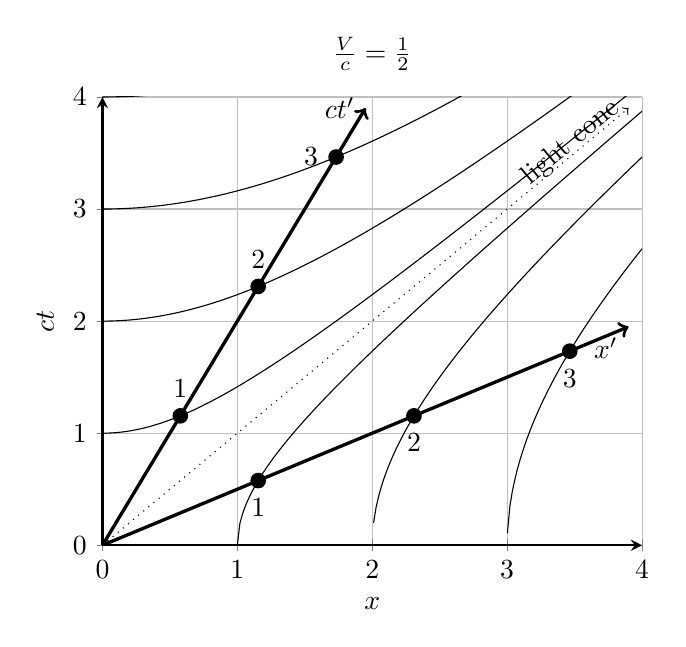
\begin{tikzpicture}
			\begin{axis}[
			axis lines=left,
			axis line style=thick,
			title={$\frac{V}{c}=\frac{1}{2}$},
			grid=both,
			xlabel = $x$,
			ylabel = {$ct$},
			legend style={at={(1.1,1)},
				anchor=north west, },
			xmin=0, xmax=4,
			ymin=0, ymax=4,
			]	
			
			%\addplot [domain=0:3.9, dotted,->] {x} node[below left] {light cone};
			\addplot [domain=0:3.9, dotted,->] {x} [allow upside down=true, yshift=5pt,sloped] node[pos=.89] {light cone};
			\addplot [very thick,domain=0:3.9,->]{x/2} [sloped] node[below left] {$x'$};
			%\addplot [very thick,domain=0:3.9,->]{x/2} [allow upside down=true, yshift=7pt, sloped] node[pos=.95] {$x'$};
			\addplot [very thick, domain=0:1.95,->] {2*x} [sloped] node[left] {$ct'$};
			\addplot [samples=500, domain=1:10]{sqrt(x^2-1)} ;
			\addplot [samples=500, domain=0:10]{sqrt(x^2+1)} ;
			\addplot [samples=500, domain=1:10]{sqrt(x^2-4)} ;
			\addplot [samples=500, domain=0:10]{sqrt(x^2+4)} ;
			\addplot [samples=500, domain=1:10]{sqrt(x^2-9)} ;
			\addplot [samples=500, domain=0:10]{sqrt(x^2+9)} ;
			\addplot [samples=500, domain=1:10]{sqrt(x^2-16)} ;
			\addplot [samples=500, domain=0:10]{sqrt(x^2+16)} ;
			\coordinate [label={below:1},circle,fill,inner sep=2pt] (x1) at (axis cs:({sqrt(4/3)},{.5*sqrt(4/3)});
			\coordinate [label={below:2},circle,fill,inner sep=2pt] (x2) at (axis cs:({2*sqrt(4/3)},{sqrt(4/3)});
			\coordinate [label={below:3},circle,fill,inner sep=2pt] (x3) at (axis cs:({3*sqrt(4/3)},{3/2*sqrt(4/3)});
			\coordinate [label={above:1},circle,fill,inner sep=2pt] (t1) at (axis cs:({.5*sqrt(4/3)},{sqrt(4/3)});
			\coordinate [label={above:2},circle,fill,inner sep=2pt] (t2) at (axis cs:({1*sqrt(4/3)},{2*sqrt(4/3)});
			\coordinate [label={left:3},circle,fill,inner sep=2pt] (t3) at (axis cs:({3/2*sqrt(4/3)},{3*sqrt(4/3)});
			%\coordinate [label=below:{$1$}] (D) at (axis cs:({sqrt(4/3)},{.5*sqrt(4/3)});
			
			
			%\addplot coordinates { ({sqrt(4/3)},{.5*sqrt(4/3)}) , (2,2)};
			%\node[label={180:{(0,1)}},circle,fill,inner sep=2pt] at (axis cs:(sqrt(4/3),.5*sqrt(4/3))) {};
			%\node[label={{(0,1)}},circle,fill,inner sep=2pt] at (axis cs:({sqrt(4/3)},{.5*sqrt(4/3)}) {};
			%\node [pin=-10:{$12$},mark=circle,draw=black] at (axis cs:{sqrt(4/3)},{.5*sqrt(4/3)}) {};
			
			\end{axis}
			\end{tikzpicture}
			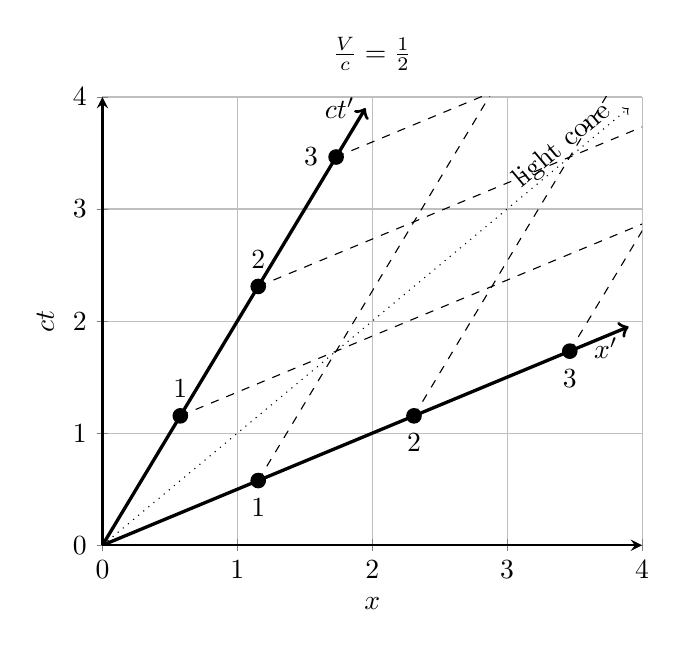
\begin{tikzpicture}
			\begin{axis}[
			axis lines=left,
			axis line style=thick,
			title={$\frac{V}{c}=\frac{1}{2}$},
			grid=both,
			xlabel = $x$,
			ylabel = {$ct$},
			legend style={at={(1.1,1)},
				anchor=north west, },
			xmin=0, xmax=4,
			ymin=0, ymax=4,
			]	
			
			%\addplot [domain=0:3.9, dotted,->] {x} node[below left] {light cone};
			\addplot [domain=0:3.9, dotted,->] {x} [every node/.style={yshift=5pt},sloped] node[pos=.89] {light cone};
			\addplot [very thick,domain=0:3.9,->]{x/2} node[below left] {$x'$};
			\addplot [very thick, domain=0:1.95,->] {2*x} node[left] {$ct'$};
			
			\addplot [dashed, domain={sqrt(4/3)}:10] {2*(x-sqrt(4/3))+.5*sqrt(4/3)};
			\coordinate [label={below:1},circle,fill,inner sep=2pt] (x1) at (axis cs:({sqrt(4/3)},{.5*sqrt(4/3)});
			
			\addplot [dashed, domain={2*sqrt(4/3)}:10] {2*(x-(2*sqrt(4/3)))+sqrt(4/3)};
			\coordinate [label={below:2},circle,fill,inner sep=2pt] (x2) at (axis cs:({2*sqrt(4/3)},{sqrt(4/3)});
			
			\addplot [dashed, domain={3*sqrt(4/3)}:10] {2*(x-(3*sqrt(4/3)))+3/2*sqrt(4/3)};
			\coordinate [label={below:3},circle,fill,inner sep=2pt] (x3) at (axis cs:({3*sqrt(4/3)},{3/2*sqrt(4/3)});
			
			\addplot [dashed, domain={.5*sqrt(4/3)}:10] {.5*(x-(.5*sqrt(4/3)))+sqrt(4/3)};
			\coordinate [label={above:1},circle,fill,inner sep=2pt] (t1) at (axis cs:({.5*sqrt(4/3)},{sqrt(4/3)});
			
			\addplot [dashed, domain={sqrt(4/3)}:10] {.5*(x-(sqrt(4/3)))+2*sqrt(4/3)};
			\coordinate [label={above:2},circle,fill,inner sep=2pt] (t2) at (axis cs:({1*sqrt(4/3)},{2*sqrt(4/3)});
			
			\addplot [dashed, domain={3/2*sqrt(4/3)}:10] {.5*(x-(3/2*sqrt(4/3)))+3*sqrt(4/3)};
			\coordinate [label={left:3},circle,fill,inner sep=2pt] (t3) at (axis cs:({3/2*sqrt(4/3)},{3*sqrt(4/3)});
			\end{axis}
			\end{tikzpicture}\\
			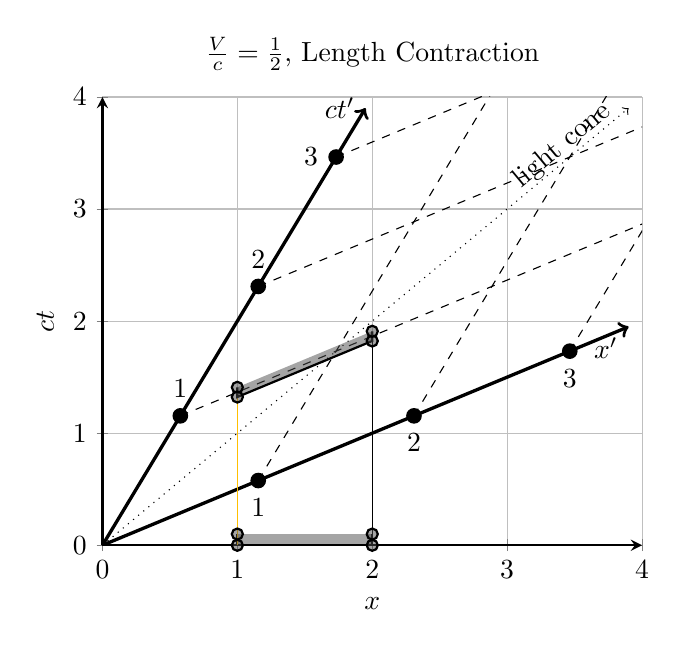
\begin{tikzpicture}
			\begin{axis}[
			axis lines=left,
			axis line style=thick,
			title={$\frac{V}{c}=\frac{1}{2}$, Length Contraction},
			grid=both,
			xlabel = $x$,
			ylabel = {$ct$},
			legend style={at={(1.1,1)},
				anchor=north west, },
			xmin=0, xmax=4,
			ymin=0, ymax=4,
			]	
			
			%\addplot [domain=0:3.9, dotted,->] {x} node[below left] {light cone};
			\addplot [domain=0:3.9, dotted,->] {x} [every node/.style={yshift=5pt},sloped] node[pos=.89] {light cone};
			\addplot [very thick,domain=0:3.9,->]{x/2} node[below left] {$x'$};
			\addplot [very thick, domain=0:1.95,->] {2*x} node[left] {$ct'$};
			
			\addplot [dashed, domain={sqrt(4/3)}:10] {2*(x-sqrt(4/3))+.5*sqrt(4/3)};
			\coordinate [label={below:1},circle,fill,inner sep=2pt] (x1) at (axis cs:({sqrt(4/3)},{.5*sqrt(4/3)});
			
			\addplot [dashed, domain={2*sqrt(4/3)}:10] {2*(x-(2*sqrt(4/3)))+sqrt(4/3)};
			\coordinate [label={below:2},circle,fill,inner sep=2pt] (x2) at (axis cs:({2*sqrt(4/3)},{sqrt(4/3)});
			
			\addplot [dashed, domain={3*sqrt(4/3)}:10] {2*(x-(3*sqrt(4/3)))+3/2*sqrt(4/3)};
			\coordinate [label={below:3},circle,fill,inner sep=2pt] (x3) at (axis cs:({3*sqrt(4/3)},{3/2*sqrt(4/3)});
			
			\addplot [dashed, domain={.5*sqrt(4/3)}:10] {.5*(x-(.5*sqrt(4/3)))+sqrt(4/3)};
			\coordinate [label={above:1},circle,fill,inner sep=2pt] (t1) at (axis cs:({.5*sqrt(4/3)},{sqrt(4/3)});
			
			\addplot [dashed, domain={sqrt(4/3)}:10] {.5*(x-(sqrt(4/3)))+2*sqrt(4/3)};
			\coordinate [label={above:2},circle,fill,inner sep=2pt] (t2) at (axis cs:({1*sqrt(4/3)},{2*sqrt(4/3)});
			
			\addplot [dashed, domain={3/2*sqrt(4/3)}:10] {.5*(x-(3/2*sqrt(4/3)))+3*sqrt(4/3)};
			\coordinate [label={left:3},circle,fill,inner sep=2pt] (t3) at (axis cs:({3/2*sqrt(4/3)},{3*sqrt(4/3)});
			
			%\addplot [fill=black!10, fill opacity=.5] coordinates {(1,.1) (1,0) (2,0) (2,.1)};
			%\addplot [circle,fill,inner sep=1pt] coordinates {(1,.1) (1,0) (2,0) (2,.1)};
			\addplot [thick,color=black!200,mark=*,fill=black!70, fill opacity=0.5] coordinates {(1,.1) (1,0) (2,0) (2,.1)};
			\addplot [mark=o]coordinates {(2,0) (2,{(.5*(2-(.5*sqrt(4/3)))+sqrt(4/3))-(sqrt(3)/40)})};			
			\addplot[mark=o, mesh] coordinates {(1,0) (1,{(.5*(1-(.5*sqrt(4/3)))+sqrt(4/3))-(sqrt(3)/40)})};
			\addplot [thick,color=black!200,mark=*,fill=black!70, fill opacity=0.5] coordinates {(1,{(.5*(1-(.5*sqrt(4/3)))+sqrt(4/3))+(sqrt(3)/40)}) (1,{(.5*(1-(.5*sqrt(4/3)))+sqrt(4/3))-(sqrt(3)/40)}) (2,{(.5*(2-(.5*sqrt(4/3)))+sqrt(4/3))-(sqrt(3)/40)}) (2,{(.5*(2-(.5*sqrt(4/3)))+sqrt(4/3))+(sqrt(3)/40)})} (1,{(.5*(1-(.5*sqrt(4/3)))+sqrt(4/3))+(sqrt(3)/40)});
			
			\end{axis}
			\end{tikzpicture}
			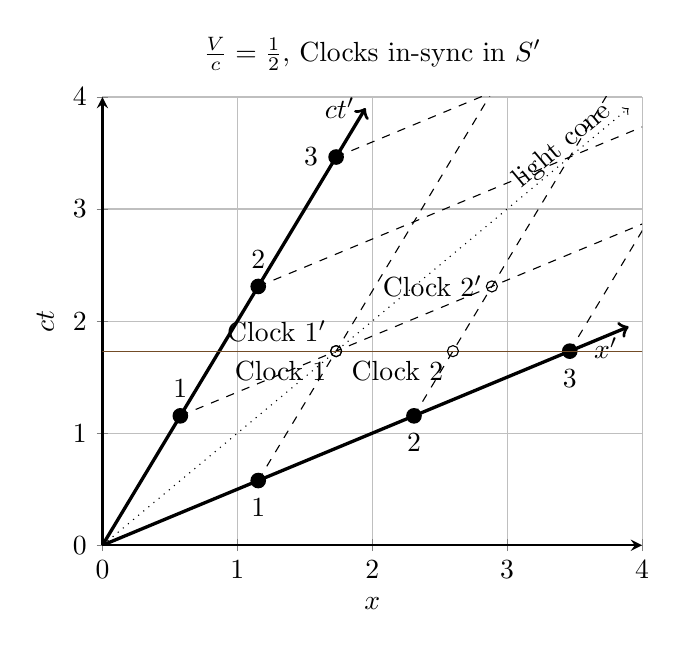
\begin{tikzpicture}
			\begin{axis}[
			axis lines=left,
			axis line style=thick,
			title={$\frac{V}{c}=\frac{1}{2}$, Clocks in-sync in $S'$},
			grid=both,
			xlabel = $x$,
			ylabel = {$ct$},
			legend style={at={(1.1,1)},
				anchor=north west, },
			xmin=0, xmax=4,
			ymin=0, ymax=4,
			]	
			
			%\addplot [domain=0:3.9, dotted,->] {x} node[below left] {light cone};
			\addplot [domain=0:3.9, dotted,->] {x} [every node/.style={yshift=5pt},sloped] node[pos=.89] {light cone};
			\addplot [very thick,domain=0:3.9,->]{x/2} node[below left] {$x'$};
			\addplot [very thick, domain=0:1.95,->] {2*x} node[left] {$ct'$};
			
			\addplot [dashed, domain={sqrt(4/3)}:10] {2*(x-sqrt(4/3))+.5*sqrt(4/3)};
			\coordinate [label={below:1},circle,fill,inner sep=2pt] (x1) at (axis cs:({sqrt(4/3)},{.5*sqrt(4/3)});
			
			\addplot [dashed, domain={2*sqrt(4/3)}:10] {2*(x-(2*sqrt(4/3)))+sqrt(4/3)};
			\coordinate [label={below:2},circle,fill,inner sep=2pt] (x2) at (axis cs:({2*sqrt(4/3)},{sqrt(4/3)});
			
			\addplot [dashed, domain={3*sqrt(4/3)}:10] {2*(x-(3*sqrt(4/3)))+3/2*sqrt(4/3)};
			\coordinate [label={below:3},circle,fill,inner sep=2pt] (x3) at (axis cs:({3*sqrt(4/3)},{3/2*sqrt(4/3)});
			
			\addplot [dashed, domain={.5*sqrt(4/3)}:10] {.5*(x-(.5*sqrt(4/3)))+sqrt(4/3)};
			\coordinate [label={above:1},circle,fill,inner sep=2pt] (t1) at (axis cs:({.5*sqrt(4/3)},{sqrt(4/3)});
			
			\addplot [dashed, domain={sqrt(4/3)}:10] {.5*(x-(sqrt(4/3)))+2*sqrt(4/3)};
			\coordinate [label={above:2},circle,fill,inner sep=2pt] (t2) at (axis cs:({1*sqrt(4/3)},{2*sqrt(4/3)});
			
			\addplot [dashed, domain={3/2*sqrt(4/3)}:10] {.5*(x-(3/2*sqrt(4/3)))+3*sqrt(4/3)};
			\coordinate [label={left:3},circle,fill,inner sep=2pt] (t3) at (axis cs:({3/2*sqrt(4/3)},{3*sqrt(4/3)});
			
			\addplot [mark=o] coordinates {({3/2*sqrt(4/3)},{3/2*sqrt(4/3)})} node[above left]{Clock $1'$};
			\addplot [mark=o] coordinates {({3/2*sqrt(4/3)},{3/2*sqrt(4/3)})} node[below left]{Clock $1$};
			\addplot [label={left:Clock 2},mark=o] coordinates {({5/2*sqrt(4/3)},{2*sqrt(4/3)})} node[left]{Clock $2'$};
			\addplot coordinates {(-1,{3/2*sqrt(4/3)}) (10,{3/2*sqrt(4/3)})};
			\addplot [label={left:Clock 2},mark=o] coordinates {({9/4*sqrt(4/3)},{3/2*sqrt(4/3)})} node[below left]{Clock $2$};
			\end{axis}
			\end{tikzpicture}\\
			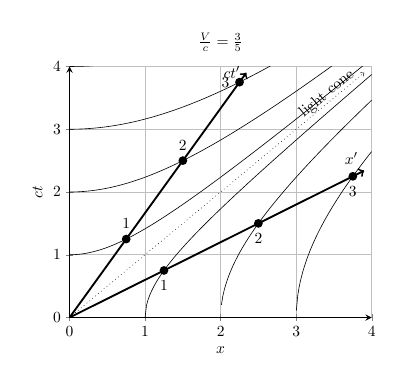
\begin{tikzpicture}[scale=.56]%[trim axis left]
			\begin{axis}[
			%scale only axis,
			%width=\textwidth*.2,
			axis lines=left,
			axis line style=thick,
			title={$\frac{V}{c}=\frac{3}{5}$},
			grid=both,
			xlabel = $x$,
			ylabel = {$ct$},
			legend style={at={(1.1,1)},
				anchor=north west, },
			xmin=0, xmax=4,
			ymin=0, ymax=4,
			]	
			
			%\addplot [domain=0:3.9, dotted,->] {x} node[below left] {light cone};
			\addplot [domain=0:3.9, dotted,->] {x} [every node/.style={yshift=5pt},sloped] node[pos=.89] {light cone};
			\addplot [very thick,domain=0:3.9,->]{3*x/5} node[above left] {$x'$};
			\addplot [very thick, domain=0:2.34,->] {5/3*x} node[left] {$ct'$};
			\addplot [samples=500, domain=1:10]{sqrt(x^2-1)} ;
			\addplot [samples=500, domain=0:10]{sqrt(x^2+1)} ;
			\addplot [samples=500, domain=1:10]{sqrt(x^2-4)} ;
			\addplot [samples=500, domain=0:10]{sqrt(x^2+4)} ;
			\addplot [samples=500, domain=1:10]{sqrt(x^2-9)} ;
			\addplot [samples=500, domain=0:10]{sqrt(x^2+9)} ;
			\addplot [samples=500, domain=1:10]{sqrt(x^2-16)} ;
			\addplot [samples=500, domain=0:10]{sqrt(x^2+16)} ;
			\coordinate [label={below:1},circle,fill,inner sep=2pt] (x1) at (axis cs:(5/4,3/4);
			\coordinate [label={below:2},circle,fill,inner sep=2pt] (x2) at (axis cs:(5/2,3/2);
			\coordinate [label={below:3},circle,fill,inner sep=2pt] (x3) at (axis cs:(15/4,9/4);
			\coordinate [label={above:1},circle,fill,inner sep=2pt] (t1) at (axis cs:(3/4,5/4);
			\coordinate [label={above:2},circle,fill,inner sep=2pt] (t2) at (axis cs:(3/2,5/2);
			\coordinate [label={left:3},circle,fill,inner sep=2pt] (t3) at (axis cs:(9/4,15/4);
			%\coordinate [label=below:{$1$}] (D) at (axis cs:({sqrt(4/3)},{.5*sqrt(4/3)});
			
			
			%\addplot coordinates { ({sqrt(4/3)},{.5*sqrt(4/3)}) , (2,2)};
			%\node[label={180:{(0,1)}},circle,fill,inner sep=2pt] at (axis cs:(sqrt(4/3),.5*sqrt(4/3))) {};
			%\node[label={{(0,1)}},circle,fill,inner sep=2pt] at (axis cs:({sqrt(4/3)},{.5*sqrt(4/3)}) {};
			%\node [pin=-10:{$12$},mark=circle,draw=black] at (axis cs:{sqrt(4/3)},{.5*sqrt(4/3)}) {};
			
			\end{axis}
			\end{tikzpicture}
			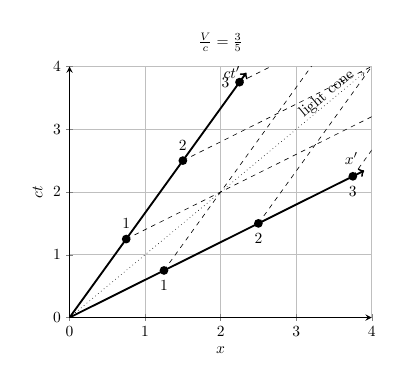
\begin{tikzpicture}[scale=.56]
			\begin{axis}[
			%scale only axis,
			%width=\textwidth*.2,
			axis lines=left,
			axis line style=thick,
			title={$\frac{V}{c}=\frac{3}{5}$},
			grid=both,
			xlabel = $x$,
			ylabel = {$ct$},
			legend style={at={(1.1,1)},
				anchor=north west, },
			xmin=0, xmax=4,
			ymin=0, ymax=4,
			]	
			
			%\addplot [domain=0:3.9, dotted,->] {x} node[below left] {light cone};
			\addplot [domain=0:3.9, dotted,->] {x} [every node/.style={yshift=5pt},sloped] node[pos=.89] {light cone};
			\addplot [very thick,domain=0:3.9,->]{3*x/5} node[above left] {$x'$};
			\addplot [very thick, domain=0:2.34,->] {5/3*x} node[left] {$ct'$};
			
			
			\addplot[dashed, domain=(5/4):10] {(5/3)*(x-(5/4))+(3/4)};
			\coordinate [label={below:1},circle,fill,inner sep=2pt] (x1) at (axis cs:(5/4,3/4);
			
			\addplot[dashed, domain=(5/2):10] {(5/3)*(x-(5/2))+(3/2)};
			\coordinate [label={below:2},circle,fill,inner sep=2pt] (x2) at (axis cs:(5/2,3/2);
			
			\addplot[dashed, domain=(15/4):10] {(5/3)*(x-(15/4))+(9/4)};
			\coordinate [label={below:3},circle,fill,inner sep=2pt] (x3) at (axis cs:(15/4,9/4);
			
			\addplot[dashed, domain=(3/4):10] {(3/5)*(x-(3/4))+(5/4)};
			\coordinate [label={above:1},circle,fill,inner sep=2pt] (t1) at (axis cs:(3/4,5/4);
			
			\addplot[dashed, domain=(3/2):10] {(3/5)*(x-(3/2))+(5/2)};
			\coordinate [label={above:2},circle,fill,inner sep=2pt] (t2) at (axis cs:(3/2,5/2);
			
			\addplot[dashed, domain=(9/4):10] {(3/5)*(x-(9/4))+(15/4)};
			\coordinate [label={left:3},circle,fill,inner sep=2pt] (t3) at (axis cs:(9/4,15/4);
			\end{axis}
			\end{tikzpicture}
			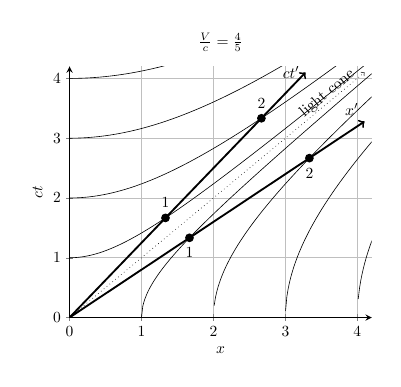
\begin{tikzpicture}[scale=.56]
			\begin{axis}[
			%scale only axis,
			%width=\textwidth*.2,
			axis lines=left,
			axis line style=thick,
			title={$\frac{V}{c}=\frac{4}{5}$},
			grid=both,
			xlabel = $x$,
			ylabel = {$ct$},
			legend style={at={(1.1,1)},
				anchor=north west, },
			xmin=0, xmax=4.2,
			ymin=0, ymax=4.2,
			]	
			
			%\addplot [domain=0:4.1, dotted,->] {x} node[below left] {light cone};
			\addplot [domain=0:4.1, dotted,->] {x} [every node/.style={yshift=5pt},sloped] node[pos=.89] {light cone};
			\addplot [very thick,domain=0:4.1,->]{4/5*x} node[above left] {$x'$};
			\addplot [very thick, domain=0:82/25,->] {5/4*x} node[left] {$ct'$};
			\addplot [samples=500, domain=1:10]{sqrt(x^2-1)} ;
			\addplot [samples=500, domain=0:10]{sqrt(x^2+1)} ;
			\addplot [samples=500, domain=1:10]{sqrt(x^2-4)} ;
			\addplot [samples=500, domain=0:10]{sqrt(x^2+4)} ;
			\addplot [samples=500, domain=1:10]{sqrt(x^2-9)} ;
			\addplot [samples=500, domain=0:10]{sqrt(x^2+9)} ;
			\addplot [samples=500, domain=1:10]{sqrt(x^2-16)} ;
			\addplot [samples=500, domain=0:10]{sqrt(x^2+16)} ;
			\coordinate [label={below:1},circle,fill,inner sep=2pt] (x1) at (axis cs:(5/3,4/3);
			\coordinate [label={below:2},circle,fill,inner sep=2pt] (x2) at (axis cs:(2*5/3,8/3);
			\coordinate [label={above:1},circle,fill,inner sep=2pt] (t1) at (axis cs:(4/3,5/3);
			\coordinate [label={above:2},circle,fill,inner sep=2pt] (t2) at (axis cs:(8/3,10/3);
			\end{axis}
			\end{tikzpicture}
			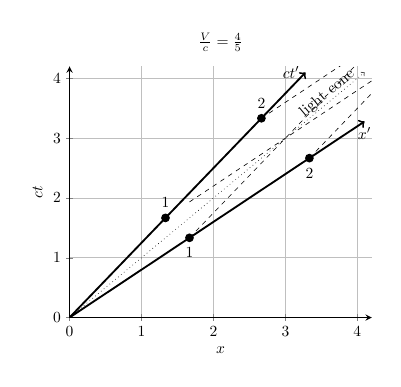
\begin{tikzpicture}[scale=.56]
			\begin{axis}[
			%scale only axis,
			%width=\textwidth*.2,
			axis lines=left,
			axis line style=thick,
			title={$\frac{V}{c}=\frac{4}{5}$},
			grid=both,
			xlabel = $x$,
			ylabel = {$ct$},
			legend style={at={(1.1,1)},
				anchor=north west, },
			xmin=0, xmax=4.2,
			ymin=0, ymax=4.2,
			]	
			
			\addplot [domain=0:4.1, dotted,->] {x} [every node/.style={yshift=5pt},sloped] node[pos=.89] {light cone};
			\addplot [very thick,domain=0:4.1,->]{4/5*x} node[below] {$x'$};
			\addplot [very thick, domain=0:82/25,->] {5/4*x} node[left] {$ct'$};
			
			%\addplot[dashed, domain=(73/55):10] {(73/48)(x-(73/55))+(48/55)};
			%\coordinate [label={below:1},circle,fill,inner sep=2pt] (x1) at (axis cs:(73/55,48/55);
			
			\addplot[dashed, domain=(5/3):10] {(5/4)*(x-(5/3))+(4/3)};
			\coordinate [label={below:1},circle,fill,inner sep=2pt] (x1) at (axis cs:(5/3,4/3);
			
			\addplot[dashed, domain=(10/3):10] {(5/4)*(x-(10/3))+(8/3)};
			\coordinate [label={below:2},circle,fill,inner sep=2pt] (x2) at (axis cs:(2*5/3,8/3);
			
			\addplot[dashed, domain=(5/3):10] {(4/5)*(x-(4/3))+(5/3)};
			\coordinate [label={above:1},circle,fill,inner sep=2pt] (t1) at (axis cs:(4/3,5/3);
			
			\addplot[dashed, domain=(8/3):10] {(4/5)*(x-(8/3))+(10/3)};
			\coordinate [label={above:2},circle,fill,inner sep=2pt] (t2) at (axis cs:(8/3,10/3);
			\end{axis}
			\end{tikzpicture}\\
		\end{center}
		%\end{multicols}
		
	\begin{description}
		\item[Invarient:] \[\left(x'\right)^2-\left(ct'\right)^2=x^2-\left(ct\right)^2=\pm a^2\]
		
		\item[Einstein's Postulates:] \hfill\begin{enumerate}
			\item Absolute uniform motion cannot be detected.
			\item The velocity of light does not depend upon the velocity of its source.
		\end{enumerate}
	\end{description}
\end{document}